\section{Introduction}
\nomenclature{AOP}{Aspect-Oriented Programming}%
\nomenclature{OOP}{Object-Oriented Programming}%

\begin{figure}
  \centering
  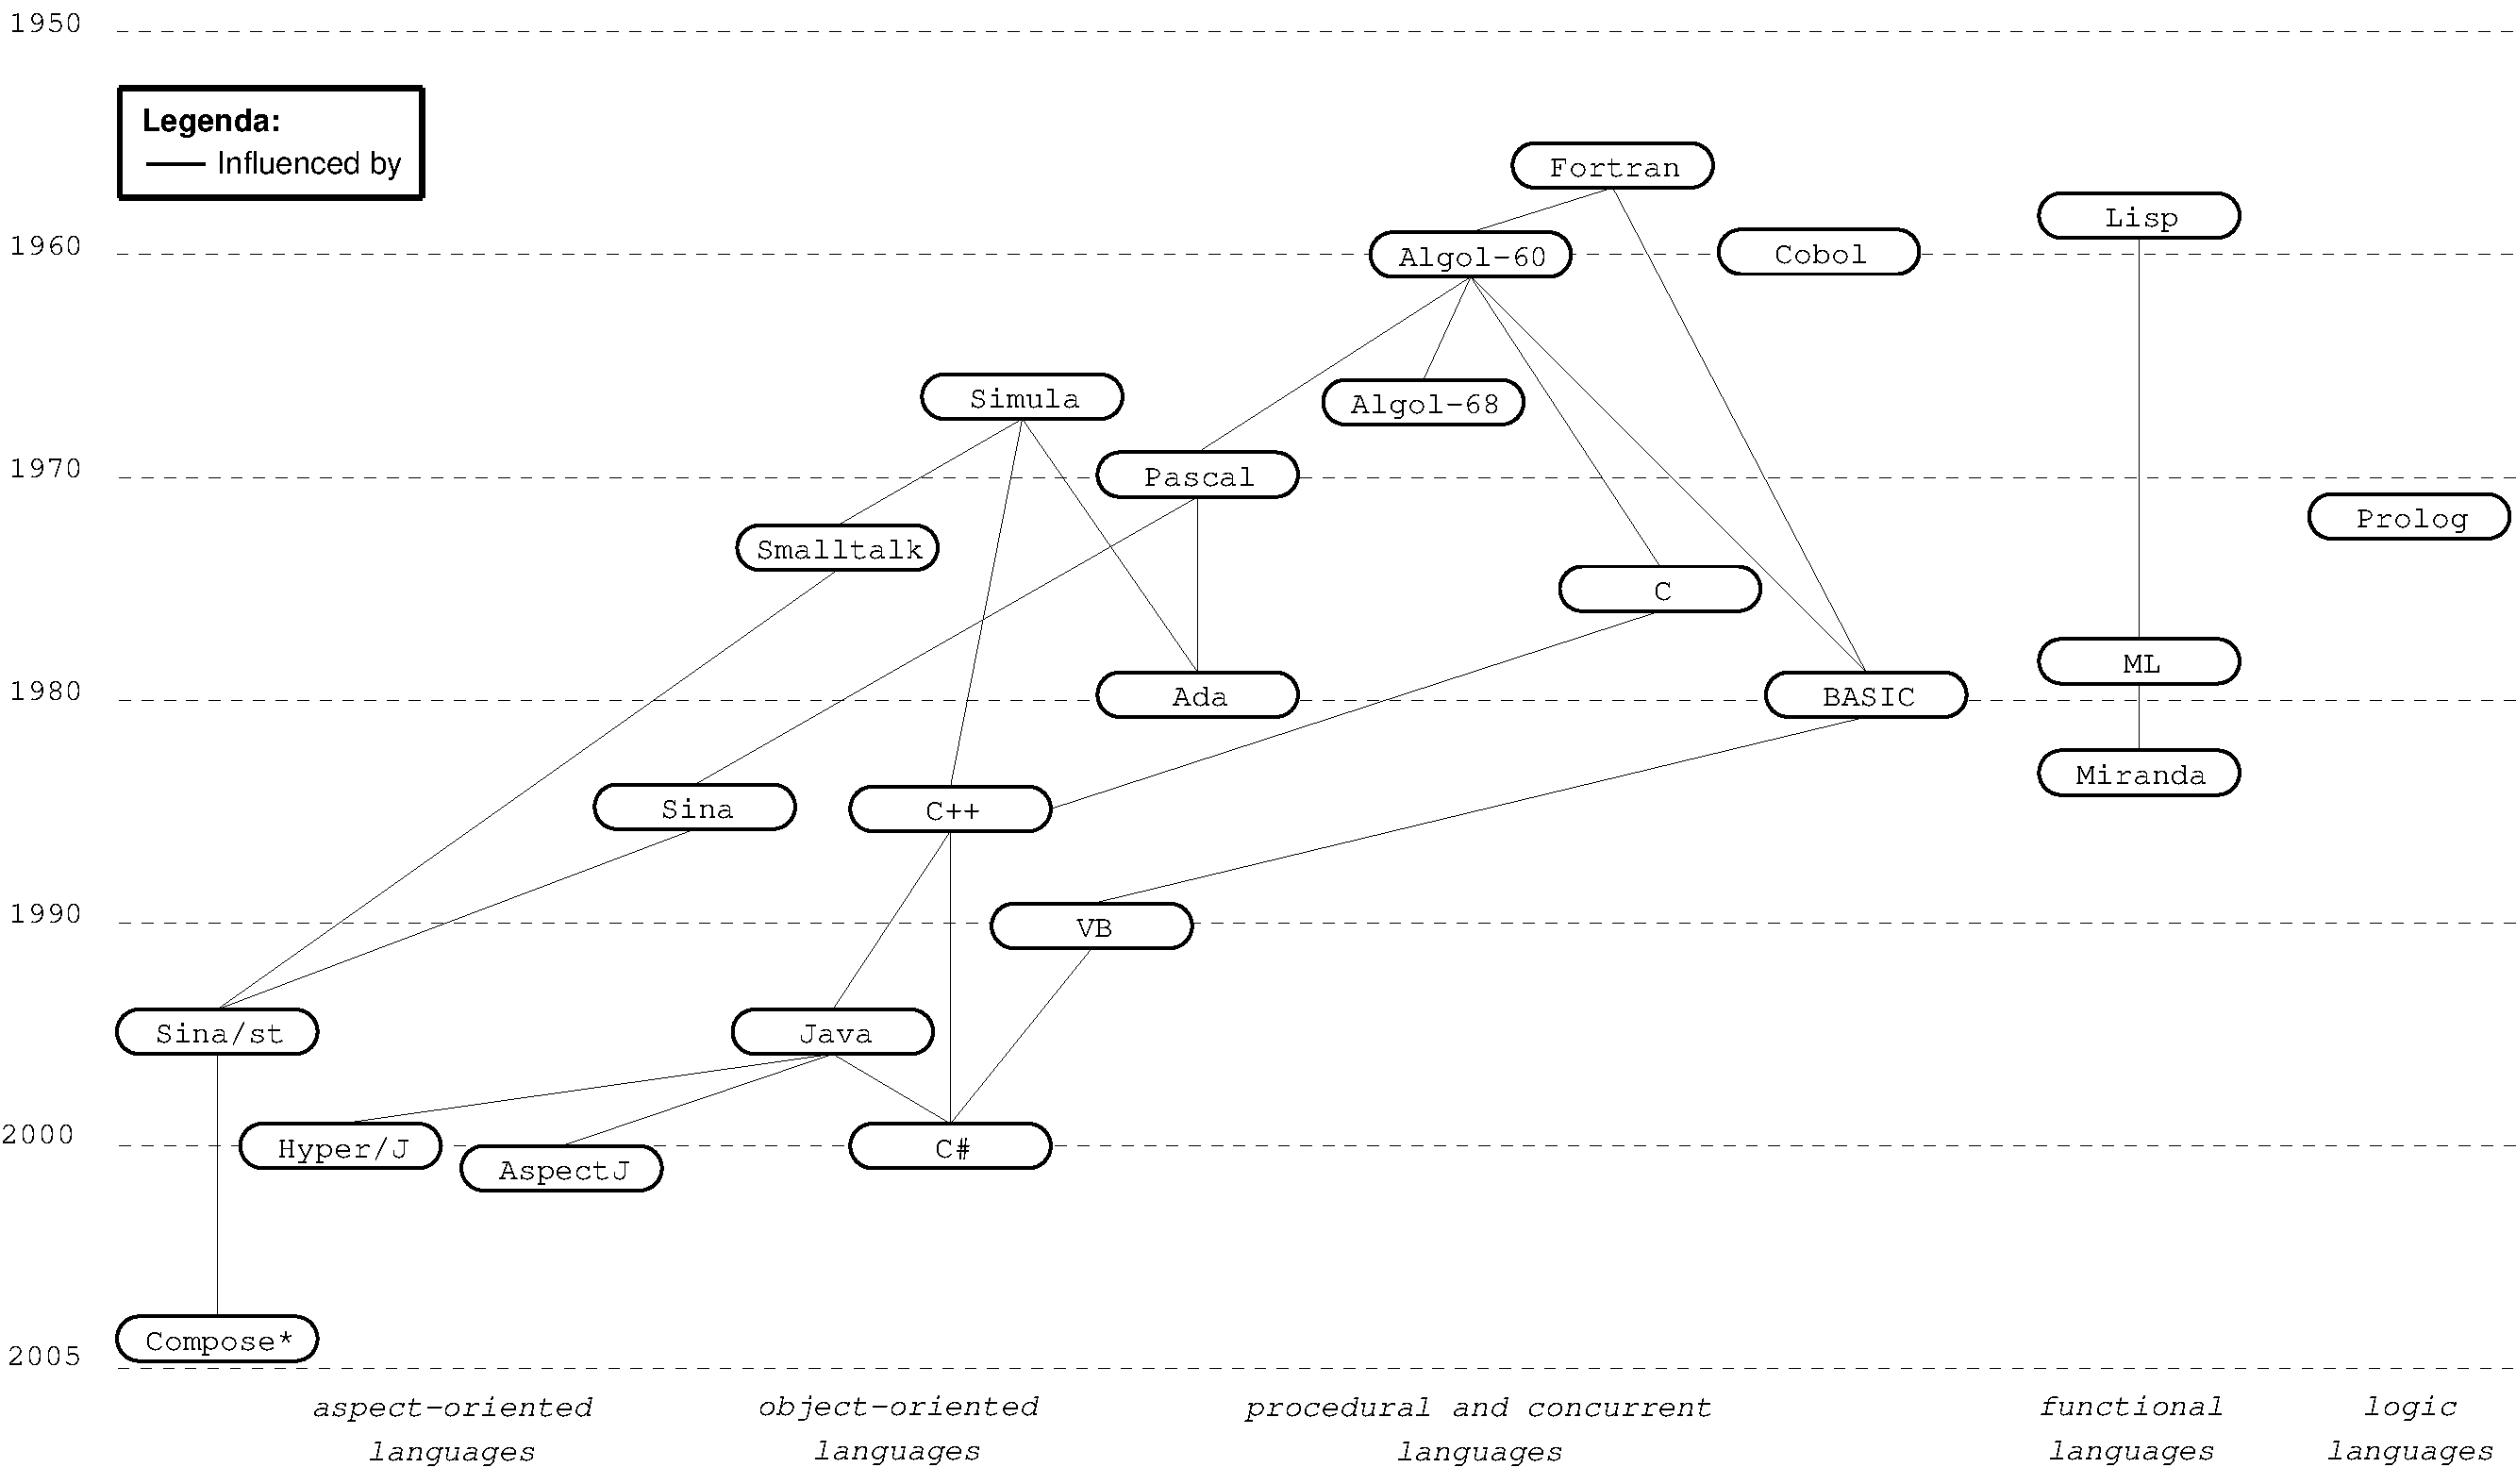
\includegraphics[style=thirdheight]{programming_languages}
  \caption{Dates and ancestry of several important languages}
  \label{fig:programming_languages}
\end{figure}

The goal of software engineering is to solve a problem by implementing a software system.
The things of interest are called concerns.
They exist at every level of the engineering process.
A recurrent theme in engineering is that of modularization: separation and localization of concerns.
The goal of modularization is to create maintainable and reusable software.
A programming language is used to implement concerns.

Fifteen years ago the dominant programming language paradigm was procedural programming.
This paradigm is characterized by the use of statements that update state variables.
Examples are Algol-like languages such as Pascal, C, and Fortran.

Other programming paradigms are the functional, logic, object-oriented, and aspect-oriented paradigms.
\autoref{fig:programming_languages} summarizes the dates and ancestry of several important languages~\cite{Watt90}.
Every paradigm uses a different modularization mechanism for separating concerns into modules.

Functional languages try to solve problems without resorting to variables.
These languages are entirely based on functions over lists and trees.
Lisp and Miranda are examples of functional languages.

A logic language is based on a subset of mathematical logic.
The computer is programmed to infer relationships between values, rather than to compute output values from input values.
Prolog is currently the most used logic language~\cite{Watt90}.

A shortcoming of procedural programming is that global variables can potentially be accessed and updated by any part of the program.
This can result in unmanageable programs because no module that accesses a global variable can be understood independently from other modules that also access that global variable.

The Object-Oriented Programming (OOP) paradigm improves modularity by encapsulating data with methods inside objects.
The data may only be accessed indirectly, by calling the associated methods.
Although the concept appeared in the seventies, it took twenty years to become popular~\cite{Watt90}.
The most well known object-oriented languages are C++, Java, C\#, and Smalltalk.

The hard part about object-oriented design is decomposing a system into objects.
The task is difficult because many factors come into play: encapsulation, granularity, dependency, adaptability, reusability, and others.
They all influence the decomposition, often in conflicting ways~\cite{Gamma95}.

Existing modularization mechanisms typically support only a small set of decompositions and usually only a single dominant modularization at a time.
This is known as the tyranny of the dominant decomposition~\cite{tarr:aosdbook05}.
A specific decomposition limits the ability to implement other concerns in a modular way.
For example, OOP modularizes concerns in classes and only fixed relations are possible.
Implementing a concern in a class might prevent another concern from being implemented as a class.

Aspect-Oriented Programming (AOP) is a paradigm that solves this problem.

AOP is commonly used in combination with OOP but can be applied to other paradigms as well.
The following sections introduce an example to demonstrate the problems that may arise with OOP and show how AOP can solve this.
Finally, we look at three particular AOP methodologies in more detail.

\section{Traditional Approach}
Consider an application containing an object \lstinline|Add| and an object \lstinline|CalcDisplay|.
\lstinline|Add| inherits from the abstract class \lstinline|Calculation| and implements its method \lstinline|execute(a, b)|. 
It performs the addition of two integers.
\lstinline|CalcDisplay| receives an update from \lstinline|Add| if a calculation is finished and prints the result to screen.
Suppose all method calls need to be traced.
The objects use a \lstinline|Tracer| object to write messages about the program execution to screen.
This is implemented by a method called \lstinline|write|.
Three concerns can be recognized: addition, display, and tracing.
The implementation might look something like \autoref{lst:calc_no_aspects}.

\begin{lstsub}
\begin{adjustwidth}{-2cm}{-2cm}%
\centering
\begin{lstsublisting}[style=listing,language=Java,escapeinside={&$}{$&},%
                      caption={Addition},label={lst:calc_no_aspects_add}]{8cm}
public class Add extends Calculation{

  private int result;
  private CalcDisplay calcDisplay;
  private Tracer trace;&$\label{line:cc_1}$&

  Add() {
    result = 0;
    calcDisplay = new CalcDisplay();
    trace = new Tracer();&$\label{line:cc_2}$&
  }

  public void execute(int a, int b) {
    trace.write("void Add.execute(int, int)");&$\label{line:cc_3}$&
    result = a + b;
    calcDisplay.update(result);
  }

  public int getLastResult() {
    trace.write("int Add.getLastResult()");&$\label{line:cc_4}$&
    return result;
  }
}
\end{lstsublisting}
\qquad
\begin{lstsublisting}[style=listing,language=Java,escapeinside={&$}{$&},%
                      caption={CalcDisplay},label={lst:calc_no_aspects_calcdisplay}]{8cm}
public class CalcDisplay {
  private Tracer trace;&$\label{line:cc_5}$&

  public CalcDisplay() {
    trace = new Tracer();&$\label{line:cc_6}$&
  }

  public void update(int value){
    trace.write("void CalcDisplay.update(int)");&$\label{line:cc_7}$&
    System.out.println("Printing new value of calculation: "+value);
  }
}
\end{lstsublisting}%
\end{adjustwidth}%
\caption{Modeling addition, display, and logging without using aspects}%
\label{lst:calc_no_aspects}%
\end{lstsub}

From our example, we recognize two forms of crosscutting: \emph{code tangling} and \emph{code scattering}.

The addition and display concerns are implemented in classes \lstinline|Add| and \lstinline|CalcDisplay| respectively.
Tracing is implemented in the class \lstinline|Tracer|, but also contains code in the other two classes (lines~\ref{line:cc_1}, \ref{line:cc_2}, \ref{line:cc_3}, and \ref{line:cc_4} in (a) and \ref{line:cc_5}, \ref{line:cc_6}, and \ref{line:cc_7} in (b)).
If a concern is implemented across several classes it is said to be scattered.
In the example of \autoref{lst:calc_no_aspects} the tracing concern is scattered.

Usually a scattered concern involves code \emph{replication}.
That is, the same code is implemented a number of times.
In our example the classes \lstinline|Add| and \lstinline|CalcDisplay| contain similar tracing code.

In class \lstinline|Add| the code for the addition and tracing concerns are intermixed.
In class \lstinline|CalcDisplay| the code for the display and tracing concerns are intermixed.
If more then one concern is implemented in a single class they are said to be tangled.
In our example the addition and tracing concerns are tangled.
Also display and tracing concerns are tangled.
Crosscutting code has the following consequences:
\begin{description}[style=nextline,noitemsep]
  \item[Code is difficult to change] Changing a scattered concern requires us to modify the code in several places.
Making modifications to a tangled concern class requires checking for side-effects with all existing crosscutting concerns;
  \item[Code is harder to reuse] To reuse an object in another system, it is necessary to either remove the tracing code or reuse the (same) tracer object in the new system;
  \item[Code is harder to understand] Tangled code makes it difficult to see which code belongs to which concern.
\end{description}

\section{AOP Approach}

To solve the problems with crosscutting, several techniques are being researched that attempt to increase the expressiveness of the OO paradigm.
Aspect-Oriented Programming (AOP) introduces a modular structure, the aspect, to capture the location and behavior of crosscutting concerns.
Examples of Aspect-Oriented languages are Sina, AspectJ, Hyper/J, and \Compose*.
A special syntax is used to specify aspects and the way in which they are combined with regular objects.
The fundamental goals of AOP are twofold~\cite{gradecki:maj03}: first to provide a mechanism to express concerns that crosscut other components.
Second to use this description to allow for the separation of concerns.

\emph{Joinpoints} are well-defined places in the structure or execution flow of a program where additional behavior can be attached.
The most common joinpoints are method calls.
\emph{Pointcuts} describe a set of joinpoints.
This allows us to execute behavior at many places in a program by one expression.
\emph{Advice} is the behavior executed at a joinpoint.

In the example of \autoref{lst:calc_aspects} the class \lstinline|Add| does not contain any tracing code and only implements the addition concern.
Class \lstinline|CalcDisplay| also does not contain tracing code.
In our example the tracing aspect contains all the tracing code.
The pointcut \lstinline|tracedCalls| specifies at which locations tracing code is executed.

\begin{lstsub}
\begin{adjustwidth}{-2cm}{-2cm}%
\centering
\begin{lstsublisting}[style=listing,language=Java,%
                      caption={Addition concern},label={lst:calc_base_add}]{75mm}
public class Add extends Calculation{
  private int result;
  private CalcDisplay calcDisplay;

  Add() {
    result = 0;
    calcDisplay = new CalcDisplay();
  }

  public void execute(int a, int b) {
    result = a + b;
    calcDisplay.update(result);
  }

  public int getLastResult() {
  	return result;
  }
}
\end{lstsublisting}\qquad
\begin{lstsublisting}[style=listing,language={[AspectJ]Java},%
                      caption={Tracing concern},label={lst:calc_trace_concern}]{85mm}
aspect Tracing {
  Tracer trace = new Tracer();

  pointcut tracedCalls(): 	 
    call(* (Calculation+).*(..)) ||
    call(* CalcDisplay.*(..));

  before(): tracedCalls() {
    trace.write(thisJoinPoint.getSignature().toString());
  }
}\end{lstsublisting}%
\end{adjustwidth}%
\caption{Modeling addition, display, and logging with aspects}%
\label{lst:calc_aspects}%
\end{lstsub}

The crosscutting concern is explicitly captured in aspects instead of being embedded within the code of other objects.
This has several advantages over the previous code.
\begin{description}[style=nextline,noitemsep]
  \item[Aspect code can be changed] Changing aspect code does not influence other concerns;
  \item[Aspect code can be reused] The coupling of aspects is done by defining pointcuts. In theory, this low coupling allows for reuse. In practice reuse is still difficult;
  \item[Aspect code is easier to understand] A concern can be understood independent of other concerns;
  \item[Aspect pluggability] Enabling or disabling concerns becomes possible.
\end{description}

\subsection{AOP Composition}
\label{sec:AOPComposition}

AOP composition can be either symmetric or asymmetric.
In the symmetric approach every component can be composed with any other component.
This approach is followed by e.g. Hyper/J.

In the asymmetric approach, the base program and aspects are distinguished.
The base program is composed with the aspects.
This approach is followed by e.g. AspectJ (covered in more detail in the next section).

\subsection{Aspect Weaving}
\label{sec:AspectWeaving}

\nomenclature{IL}{Intermediate Language}%
\nomenclature{CIL}{Common Intermediate Language}%
The integration of components and aspects is called \emph{aspect weaving}.
There are three approaches to aspect weaving.
The first and second approach rely on adding behavior in the program, either by weaving the aspect in the source code, or by weaving directly in the target language.
The target language can be intermediate language (IL) or machine code.
Examples of IL are Java byte code and Common Intermediate Language (CIL).
The remainder of this chapter considers only intermediate language targets.
The third approach relies on adapting the virtual machine.
Each method is explained briefly in the following sections.

\subsubsection{Source Code Weaving}
\label{sec:source_code_weaving}

The source code weaver combines the original source with aspect code.
It interprets the defined aspects and combines them with the original source, generating input for the native compiler.
For the native compiler there is no difference between source code with and without aspects.
Hereafter the compiler generates an intermediate or machine language output (depending on the compiler-type).

The advantages of using source code weaving are:
\begin{description}[style=nextline,noitemsep]
  \item[High-level source modification] Since all modifications are done at source code level, there is no need to know the target (output) language of the native compiler;
  \item[Aspect and original source optimization] First the aspects are woven into the source code and hereafter compiled by the native compiler.
       The produced target language has all the benefits of the native compiler optimization passes.
       However, optimizations specific to exploiting aspect knowledge are not possible;
  \item[Native compiler portability] The native compiler can be replaced by any other compiler as long as it has the same input language.
       Replacing the compiler with a newer version or another target language can be done with little or no modification to the aspect weaver.
\end{description}

However, the drawbacks of source code weaving are:
\begin{description}[style=nextline,noitemsep]
  \item[Language dependency] Source code weaving is written explicitly for the syntax of the input language;
  \item[Limited expressiveness] Aspects are limited to the expressive power of the source language.
       For example, when using source code weaving, it is not possible to add multiple inheritance to a single inheritance language.
\end{description}

\subsubsection{Intermediate Language Weaving}
\label{sec:intermediate_language_weaving}

Weaving aspects through an intermediate language gives more control over the executable program and solves some issues as identified in \autoref{sec:source_code_weaving} on source code weaving.
Weaving at this level allows for creating combinations of intermediate language constructs that can not be expressed at the source code level.
Although IL can be hard to understand, IL weaving has several advantages over source code weaving:
\begin{description}[style=nextline,noitemsep]
  \item[Programming language independence] All compilers generating the target IL output can be used;
  \item[More expressiveness] It is possible to create IL constructs that are not possible in the original programming language;
  \item[Source code independence] Can add aspects to programs and libraries without using the source code (which may not be available);
  \item[Adding aspects at load- or runtime] A special class loader or runtime environment can decide and do dynamic weaving.
       The aspect weaver adds a runtime environment into the program.
       How and when aspects can be added to the program depend on the implementation of the runtime environment.
\end{description}

However, IL weaving also has drawbacks that do not exist for source code weaving:
\begin{description}[style=nextline,noitemsep]
  \item[Hard to understand] Specific knowledge about the IL is needed;
  \item[More error-prone] Compiler optimization may cause unexpected results.
       Compiler can remove code that breaks the attached aspect (\eg inlining of methods).
\end{description}

\subsubsection{Adapting the Virtual Machine}

\nomenclature{VM}{Virtual Machine}%
Adapting the virtual machine (VM) removes the need to weave aspects.
This technique has the same advantages as intermediate language weaving and can also overcome some of its disadvantages as mentioned in \autoref{sec:intermediate_language_weaving}.
Aspects can be added without recompilation, redeployment, and restart of the application~\cite{popovici:aosd02,popovici:aosd03}.

Modifying the virtual machine also has its disadvantages:
\begin{description}[style=nextline,noitemsep]
  \item[Dependency on adapted virtual machines] Using an adapted virtual machine requires that every system should be upgraded to that version;
  \item[Virtual machine optimization] People have spend a lot of time optimizing virtual machines.
       By modifying the virtual machine these optimizations should be revisited.
       Reintegrating changes introduced by newer versions of the original virtual machine, might have substantial impact.
\end{description}

